\textbf{Example}

Xét lần gọi hàm sau:

\begin{lstlisting}
solve(6, 2, 2, {0, 0, 0, 1, 2}, {1, 2, 5, 3, 4}, {3, 4}, {1, 2}, {5, 5}, {0, 1})
\end{lstlisting}

Hệ thống đô thị của thành phố XYZ bao gồm $N=6$ khu dân cư và có thể được mô phỏng theo hình như sau:

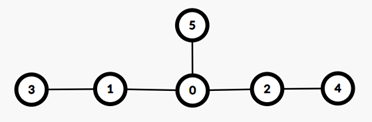
\includegraphics{tst2026-p1-example.png}

Có $K=2$ tuyến đường được ban quy hoạch đô thị chọn làm tuyến đường trọng điểm. Các tuyến đường đó bao gồm:
\begin{itemize}
   \item $3 - 1$
   \item $4 - 2$
\end{itemize}

Ban quy hoạch đô thị sẽ xét tuyến đường tiềm năng trong $Q=2$ ngày tiếp theo:
\begin{itemize}
   \item Trong ngày thứ $0$, tuyến đường tiềm năng là tuyến đường $5 - 0$. Có thể đặt $3$ trạm tại các khu dân cư $3,4,5$ để thỏa mãn yêu cầu đề bài.
   \item Trong ngày thứ $1$, tuyến đường tiềm năng là tuyến đường $5 - 0 - 1$. Có thể đặt $2$ trạm tại các khu dân cư $1,2$ để thỏa mãn yêu cầu đề bài.
   \item Có thể chứng minh không có phương án nào cho ra kết quả tối ưu hơn.
\end{itemize}

Như vậy, hàm trên cần trả về kết quả là $\{3,2\}$.